\chapter[Algoritmo]{Algoritmo}
\label{ch:algoritmo}

\section{Preprocesamiento de la base de datos}
\label{sec:proc_bdd}
	\subsection{Detección de rostros}
	\label{algoritmo:det_rostro}
	
	\subsection{Corrección de movimiento}
	\label{algoritmo:cor_movimiento}

\section{Extracción de micro-descriptores}
\label{sec:micro-descriptores}
		El proceso de extracción de micro-descriptores es el núcleo del algoritmo. Este proceso es el encargado de la extracción de características directas del vídeo o imagen dinámica. Para esto se introduce un nuevo término que es denominado ``Rayo de flujo'' o simplemente ``Rayo''. Éste define cual es el movimiento de las regiones de interés (ROI sigla en ingles) en los cuadros del vídeo.

	\subsection{Elección de regiones de interés}
	\label{algoritmo:elecc_roi}
	Para cada uno de los vídeos que se quiere procesar, después de realizar el preprocesamiento definido en la Sección~\ref{sec:proc_bdd}. Se seleccionan las regiones de interés a las cuales se les quiere extraer los ``Rayos''. Las áreas son seleccionadas dependiendo de la cantidad de información que entregan. 
	
	Se define un vídeo 
	\begin{equation}\label{algoritmo:eq:video}		
		V = \{Roi_i~|~\forall ~1~\leq~i~\le~N\}, 
	\end{equation}
	donde $N$ es el número de regiones de interés en el vídeo.
	
	Se define un ROI, $R_i$ como
	\begin{equation}\label{algoritmo:eq:roi}
		Roi_i = \{(x,y,t) | (x,y,y) \in \mathds{R}(N)\},
	\end{equation}
	Donde $\mathds{R}(N)$, es la función que indica en cuantas regiones se divide la imagen.

	\subsection{Extracción de rayos}
	\label{algoritmo:ext_rayos}
	Para esta sección se introducen dos términos, la región de soporte y ventana de búsqueda.
	\paragraph{Región de soporte.} es una sección de la ROI la cual es de tamaño $T$, donde $T$ es impar y esta centrada en el píxel $(x,y)$ en el cuadro $t$ del vídeo. Esta región es utilizada para calcular el movimiento de dicho píxel con respecto al cuadro $t+1$.
	\paragraph{Ventana de búsqueda.} al igual que la región de soporte es una sección del ROI de tamaño $2T+1$ y centrada en el píxel $(x,y)$, pero a diferencia de la anterior, esta se extrae del cuadro $t+1$. El objetivo de esta ventana es generar un espacio supuesto, donde se puede haber desplazo la región de soporte.
		
	La extracción de rayos consiste en que para cada píxel de la región de interés, se obtenga una región de soporte en cada cuadro y esta sea buscada dentro de la ventana de búsqueda del cuadro siguiente. Esta búsqueda se realiza calculando el error Cuadrático Medio o MSE (por sus siglas en ingles), \begin{equation}\label{algoritmo:eq:mse}	
			MSE(\mathit{RS},\mathit{RS'}) = \sum_{x=1}^{T} \sum_{y=1}^{T} (\mathit{RS}(x,y) - \mathit{RS'}(x,y))^2,
		\end{equation} 
	para cada uno de los desplazamientos que se puedan realizar de la región de soporte sobre la de búsqueda. Luego de calcular el MSE de cada píxel dentro de la región de búsqueda se procede a calcular el minMSE
	\begin{equation}
		RS^* = argmin\{MSE(RS,RS') | RS' \in WS\},
	\end{equation}		
	el cual será el cuadro donde la ventana de soporte se desplazó en el cuadro $t+1$, con esto se obtiene el píxel $(x',y')$ que corresponde al centro de la ventana obtenida en el proceso anterior.
	
	Para calcular el desplazamiento en el cuadro $t$ de $(x,y)$ a $(x',y')$, se procede a realizar la resta de los ejes. De tal forma que
	\begin{equation}
		\Delta x = x-x', 
	\end{equation}		
	\begin{equation}
		\Delta y = y-y'.
	\end{equation}		
	Estos $ \Delta x$ y $ \Delta y$ son definidos como ``Rayos de soporte''
	\begin{equation}
		\rho_j = \{(\Delta x_j, \Delta y_j)~|~j~es~el~numero~de~píxeles~en~la~region~RS \}
	\end{equation}		
	 y son la estructura básica de los ``Rayos de flujo'', dado que al juntar todos los desplazamientos del píxel $(x,y)$ a lo largo de los cuadros del vídeo, se obtiene un conjunto de variaciones de movimientos de estos, este conjunto es definido como el ``Rayo'' o micro-descriptor.
	\begin{equation}
		R^i_l	 = \{\rho_j | ~\forall ~1~\leq~i~\le~j\ \wedge R^i_l \in Roi_i \}
	\end{equation}
		
		%%HABLAR DE ventana de soporte, ventana de busqueda MSE
		
	\subsection{Normalización de rayos}
	\label{algoritmo:normalizacion}
	Luego de obtener el total de micro-descriptores es necesario poder llevar todos los rayos al mismo espacio vectorial, esto debido a el tamaño de cada conjunto depende la cantidad de cuadros $F$ del vídeo. Para este proceso se introduce una variable muy importante para el algoritmo llamada $N$, esta sera la encargada de comandar el proceso de normalización, de tal forma que se obtiene una razón de normalización
	\begin{equation}
		Razon = \frac{F}{N},
	\end{equation}
	que permite relacionar la cantidad de ``Rayos de soporte'' $\rho_j$ del ``Rayo'' $R^i_l$ original formaran parte de los $\rho_j '$ de $R^{i'}_l$' normalizado. Este proceso puede ser visualizado en la Figura~\ref{algoritmo:fig:normalizacion}
	
	\begin{figure}[!]
		\centering
  		\label{algoritmo:fig:normalizacion}
    		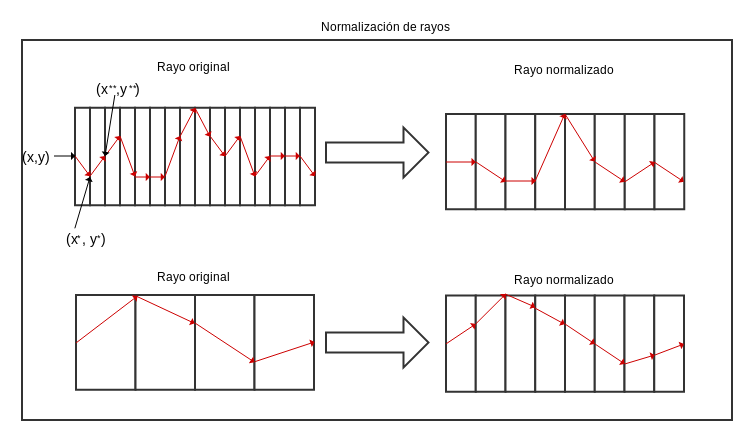
\includegraphics[width=1\textwidth]{Figuras/Diagramas/normalizacion_de_rayos.png}
  		\caption{Normalización de rayos.}
	\end{figure}	

	
\newpage	
\section{Creación de macro-descriptores}
\label{sec:macro-descriptores}
El proceso de creación de macro-descriptores es el proceso final de la extracción de características de los vídeos. Luego de obtener un extenso conjunto de ``Rayos'' para cada uno de los vídeos, es necesario poder crear grupos de ``rayos'', los cuales puedan representar de mejor manera el espacio ya normalizado. Para esto se utilizan técnicas de ``clustering'' o agrupamiento.
	\subsection{Bag of words}
	\label{algoritmo:bow}
		Esta es una técnica dependiente de la cantidad de palabras $K$ o ``words'' se introduzcan a la bolsa, esta técnica permite armar $K$ grupos representados cada uno de estos por un centroide o ``cluster'' llamado $C_k$ como se puede ver en la Figura~\ref{algoritmo:fig:bow}. Estos son los puntos de referencia de cada uno de sus grupos, para saber a cual de estos $k$ centroides pertenece un ``Rayo'' $R^{i'}_l$, es necesario calcular el
		\begin{equation}
  			\label{algoritmo:eq:dist}
			k^* = Argmin\{dist(R^{i'}_l,C_k)\},
		\end{equation}
		donde la función de distancia $dist()$ a utilizar depende de la instancia del algoritmo.

	\begin{figure}[h]
		\centering
  		\label{algoritmo:fig:bow}
    		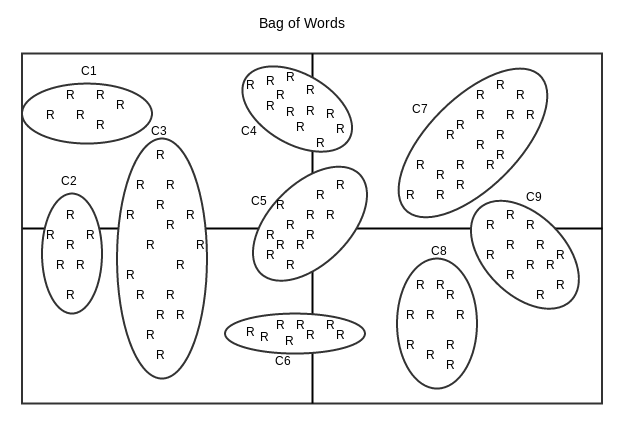
\includegraphics[width=1\textwidth]{Figuras/Diagramas/bow_solo.png}
  		\caption{Construcción del Bag of Words.}
	\end{figure}	
La variable $K$ es muy importante a la hora de su elección, esto debido a la gran cantidad de micro-descriptores extraídos en el paso anterior. La cantidad de agrupaciones a formar sera un tema abordado de forma mayoritaria en el Capitulo~\ref{ch:exp_result}.

	\subsection{Creación de macro-descriptores}
	\label{algoritmo:crea_macro-descriptores}
	Luego de tener etiquetado cada uno de los ``Rayos'' $R^{i'}_l$ con su centroide respectivo, se procede a crear el macro-descriptor de cada uno de los vídeos.	 Se crea un histograma de tamaño $K$ para cada uno de las regiones de interés $Roi_i$ del vídeo, de tal forma que en este histograma se tenga presente la frecuencia de cada uno de los clusters encontrados en la creación del Bag of Words. Luego de obtener dichos descriptores por región, se procede a juntar o concatenar cada uno de los histogramas pertenecientes al mismo vídeo, este proceso puede ser visto en la Figura~\ref{algoritmo:fig:macro-descriptores}. El resultado de esta concatenación es el macro-descriptor del vídeo seleccionado.
	\begin{figure}[h]
		\centering
  		\label{algoritmo:fig:macro-descriptores}
    		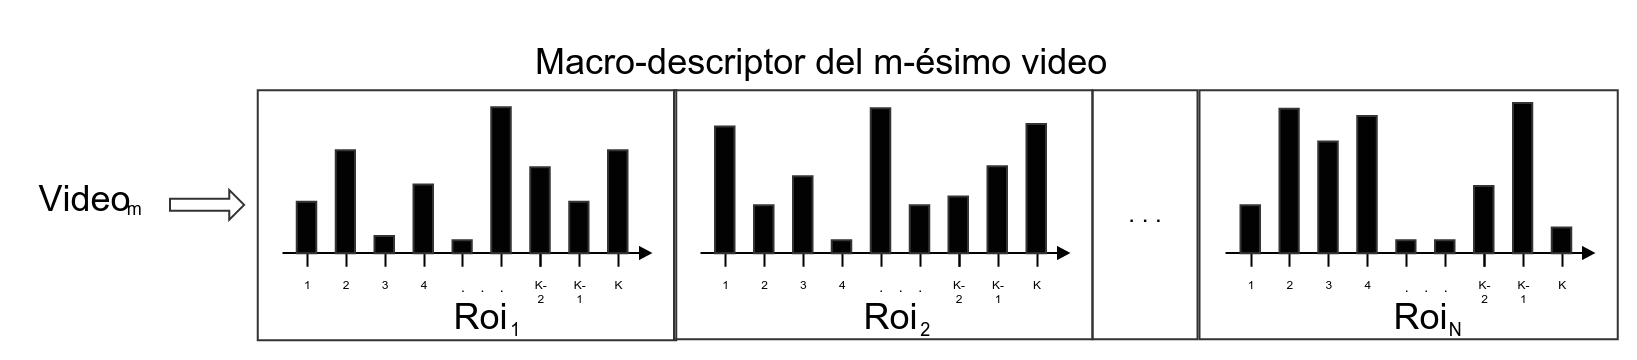
\includegraphics[width=1\textwidth]{Figuras/Diagramas/macro-descriptor.png}
  		\caption{Construcción del macro-descriptor.}
	\end{figure}	

	En el proceso clasificación, no se recalculan los centroides para un nuevo vídeo, ya que, se guarda el modelo que contiene el resultado del Bag of Words, y se procede a calcular~\ref{algoritmo:eq:dist}, para cada uno de los ``Rayos'' $R^{i'}_l$ obtenidos en el proceso de extracción de micro-descriptores. Luego de esto al igual que en el proceso de entrenamiento se crea el macro-descriptor con el mismo método.
	
	
\section{Entrenamiento y clasificación}
\label{sec:clasificacion}

	\subsection{Entrenamiento}
	\label{algoritmo:entrenamiento}
	
	\subsection{Clasificación}
	\label{algoritmo:clasificacion}
	
	
	
	
	
	
	